\section{Dotplots \cite{wiki-dotplot,ism-2}}\label{dotplots}
\begin{enumerate}
    \item A dotplot is an attractive summary of numerical data when the data set is reasonably small or there are relatively few distinct data values. 
    \item Each observation is represented by a dot above the corresponding location on a horizontal measurement scale. 
    \item When a value occurs more than once, there is a dot for each occurrence, and these dots are stacked vertically
    \item A dotplot gives information about location, spread, extremes, and gaps
\end{enumerate}

\begin{figure}
    \centering
    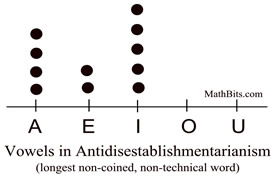
\includegraphics[height=3cm]{Pictures/data/data_dotplot.jpg}
    \caption{Graph: Dotplot}
\end{figure}
